\begin{ghichu}
\textbf{Lưu ý bắt buộc khi đọc chương này:} toàn bộ số liệu trong Chương 6 là \textbf{kết quả mô phỏng} với N = 30 lần chạy cho mỗi tổ hợp, tổng cộng 180 lần chạy. Đây \textbf{không phải} số liệu đo trên robot thật. Mọi hình vẽ trong chương đều ghi lại điều này ở chân hình.
\end{ghichu}

\subsection{Bảng kết quả tổng hợp}
\begin{table}[!htbp]
  \centering
  \caption{Kết quả mô phỏng tổng hợp --- 3 thuật toán $\times$ 2 môi trường $\times$ 30 lần chạy}
  \small
  \renewcommand{\arraystretch}{1.25}
  \begin{tabular}{>{\raggedright\arraybackslash}p{0.1653\textwidth}>{\raggedright\arraybackslash}p{0.1405\textwidth}>{\raggedright\arraybackslash}p{0.1405\textwidth}>{\raggedright\arraybackslash}p{0.1322\textwidth}>{\raggedright\arraybackslash}p{0.1240\textwidth}>{\raggedright\arraybackslash}p{0.1240\textwidth}}
    \toprule
    \textbf{Thuật toán} & \textbf{Môi trường} & \textbf{Thời gian (s)} & \textbf{Quãng đường (m)} & \textbf{Sai số (cm)} & \textbf{Thành công} \\
    \midrule
    Quét toàn bộ & Khuếch tán & 273,6 $\pm$ 7,1 & 16,53 $\pm$ 0,82 & 22,7 $\pm$ 10,0 & 23/30 (77 \%) \\
    Bám gradient & Khuếch tán & 106,8 $\pm$ 29,9 & 4,17 $\pm$ 1,13 & 26,0 $\pm$ 12,9 & 20/30 (67 \%) \\
    Surge-casting & Khuếch tán & 95,3 $\pm$ 25,4 & 4,36 $\pm$ 0,97 & 50,1 $\pm$ 23,1 & 5/30 (17 \%) \\
    Quét toàn bộ & Đứt quãng & 266,8 $\pm$ 8,8 & 15,63 $\pm$ 1,01 & 34,2 $\pm$ 23,3 & 19/30 (63 \%) \\
    Bám gradient & Đứt quãng & 98,0 $\pm$ 42,4 & 4,43 $\pm$ 2,23 & 72,2 $\pm$ 43,9 & 5/30 (17 \%) \\
    Surge-casting & Đứt quãng & 145,5 $\pm$ 67,7 & 9,16 $\pm$ 4,97 & 44,0 $\pm$ 35,9 & 17/30 (57 \%) \\
    \bottomrule
  \end{tabular}
\end{table}
Các giá trị trình bày dưới dạng trung bình $\pm$ độ lệch chuẩn. Khoảng tin cậy 95 \% cho tỉ lệ thành công (theo phương pháp Wilson) lần lượt là: 59--88 \%, 49--81 \%, 7--34 \% cho môi trường khuếch tán và 46--78 \%, 7--34 \%, 39--73 \% cho môi trường đứt quãng.


\subsection{Tỉ lệ thành công}
\begin{figure}[!htbp]
  \centering
  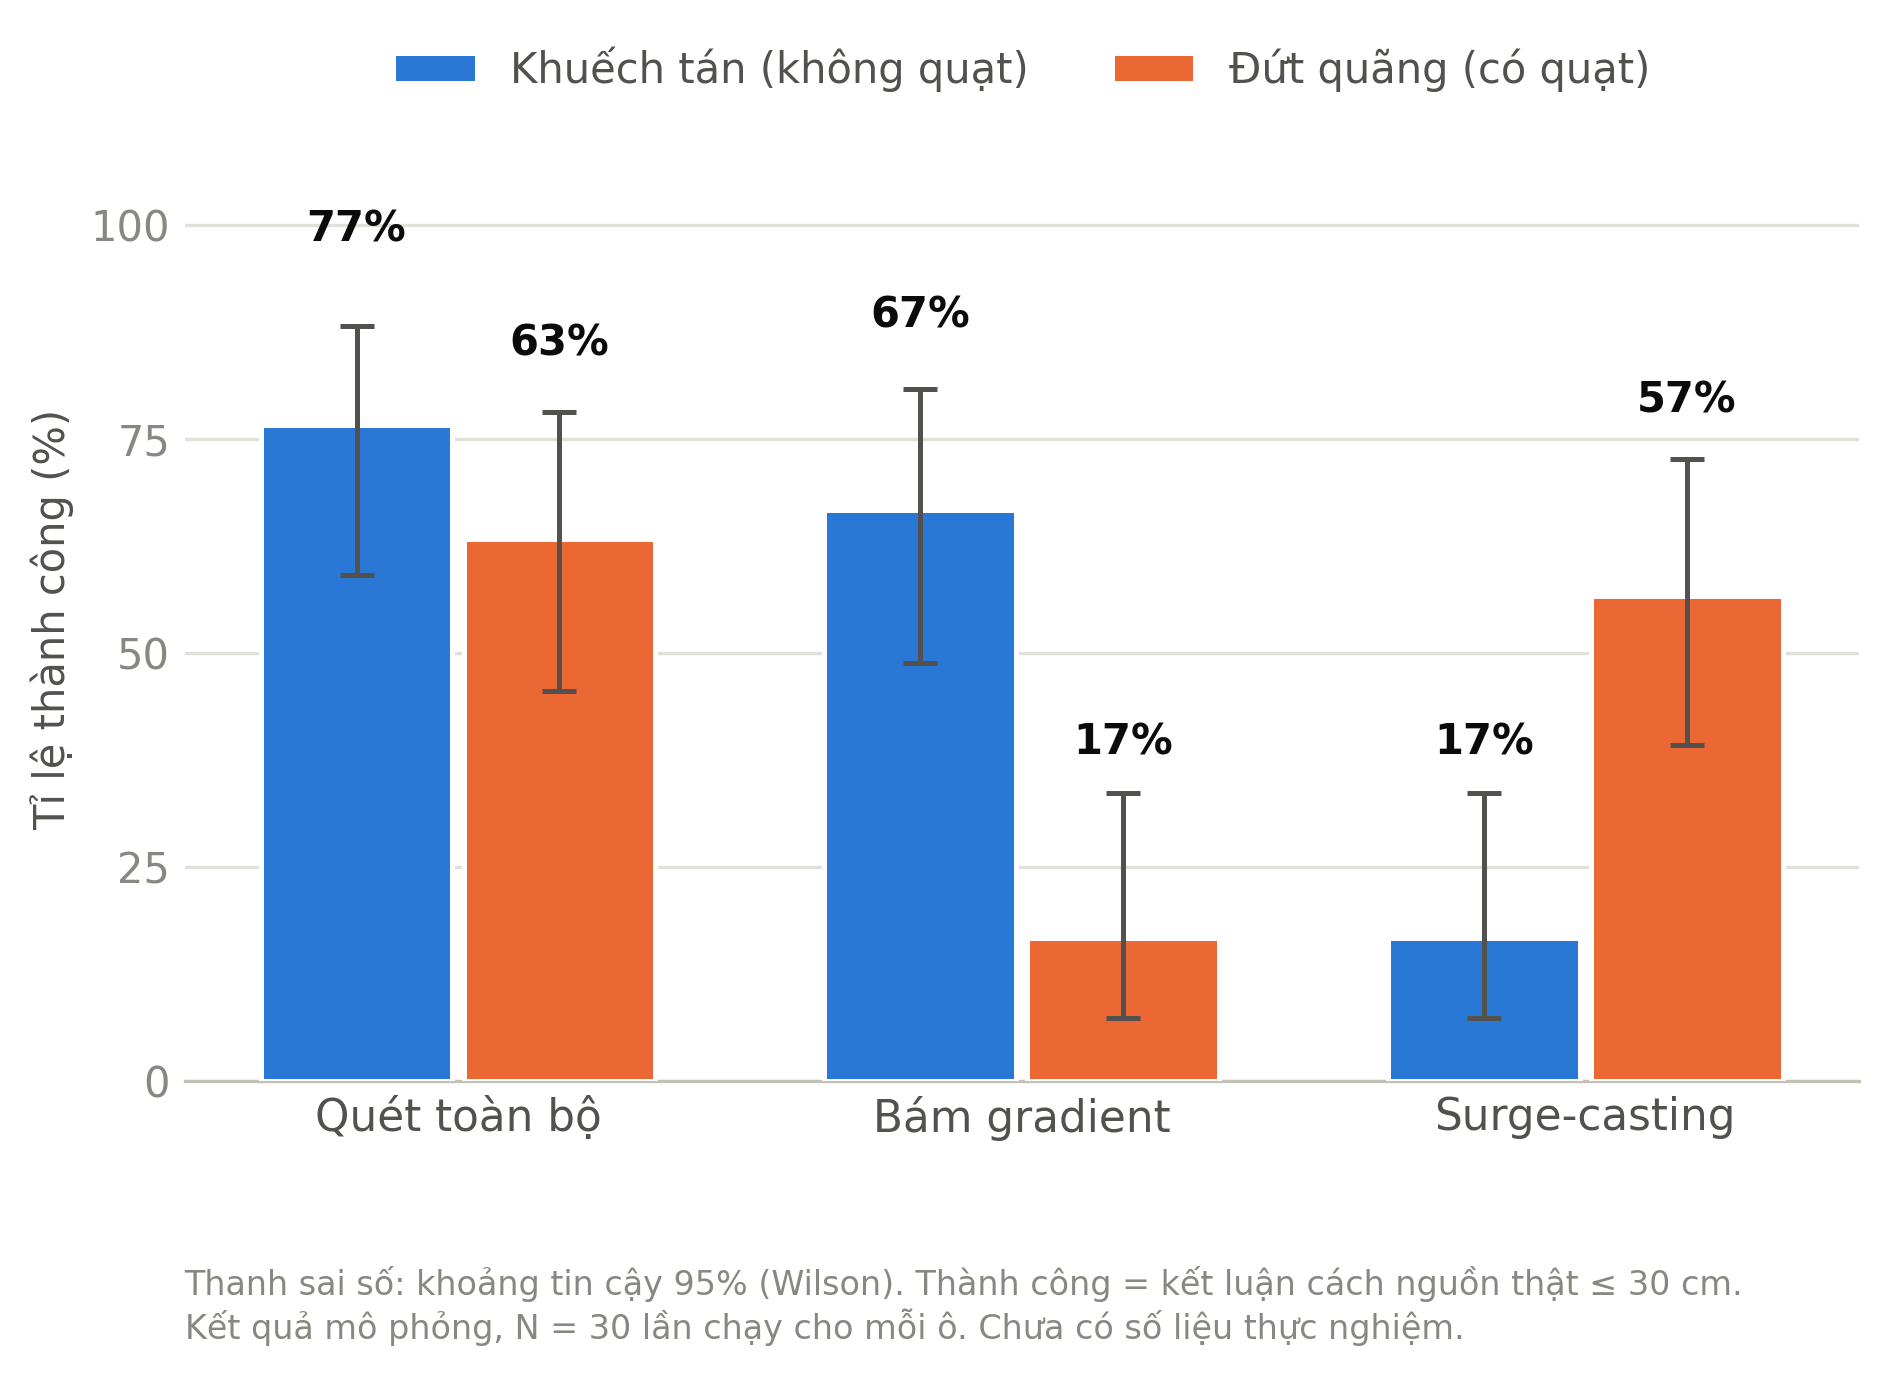
\includegraphics[width=0.912\textwidth]{pic/kq1_thanhcong.png}
  \caption{Tỉ lệ thành công của ba thuật toán trong hai môi trường. Hiệu ứng đảo chiều giữa bám gradient và surge-casting là kết quả chính của đề tài.}
\end{figure}
Hình 6.1 cho thấy kết quả trung tâm của toàn bộ đề tài: \textbf{hai thuật toán ``thông minh'' đảo chiều nhau khi đổi môi trường}, trong khi thuật toán mốc gần như không đổi.

\begin{itemize}[leftmargin=1.4em,itemsep=0.15em,topsep=0.3em]
  \item Trong môi trường \textbf{khuếch tán}, bám gradient đạt 67 \% còn surge-casting chỉ đạt 17 \%.
  \item Trong môi trường \textbf{đứt quãng}, tình thế đảo ngược hoàn toàn: bám gradient rơi xuống 17 \% còn surge-casting lên 57 \%.
  \item Quét toàn bộ giữ ở 77 \% và 63 \%, không thay đổi đáng kể.
\end{itemize}
Cả hai chiều đảo đều \textbf{có ý nghĩa thống kê} (xem mục 6.6). Điều đáng chú ý là hiệu ứng này không phải một chênh lệch nhỏ cần phải nhìn kỹ mới thấy: tỉ lệ thành công thay đổi gần bốn lần theo cả hai chiều.

Ý nghĩa vật lý của từng chiều đã được dự đoán từ Chương 2 và đúng như dự đoán. Bám gradient cần một trường nồng độ trơn và giảm đơn điệu; môi trường khuếch tán cung cấp đúng điều đó, còn môi trường đứt quãng thì phá huỷ nó. Ngược lại, surge-casting cần một hướng gió xác định được; môi trường đứt quãng có quạt cung cấp đúng điều đó, còn môi trường khuếch tán thì \textbf{không có gió}, nên khái niệm ``đi ngược hướng gió'' mất hết ý nghĩa và robot chỉ đi theo một hướng khai báo cứng, gần như ngẫu nhiên so với vị trí nguồn thật.


\subsection{Thời gian định vị}
\begin{figure}[!htbp]
  \centering
  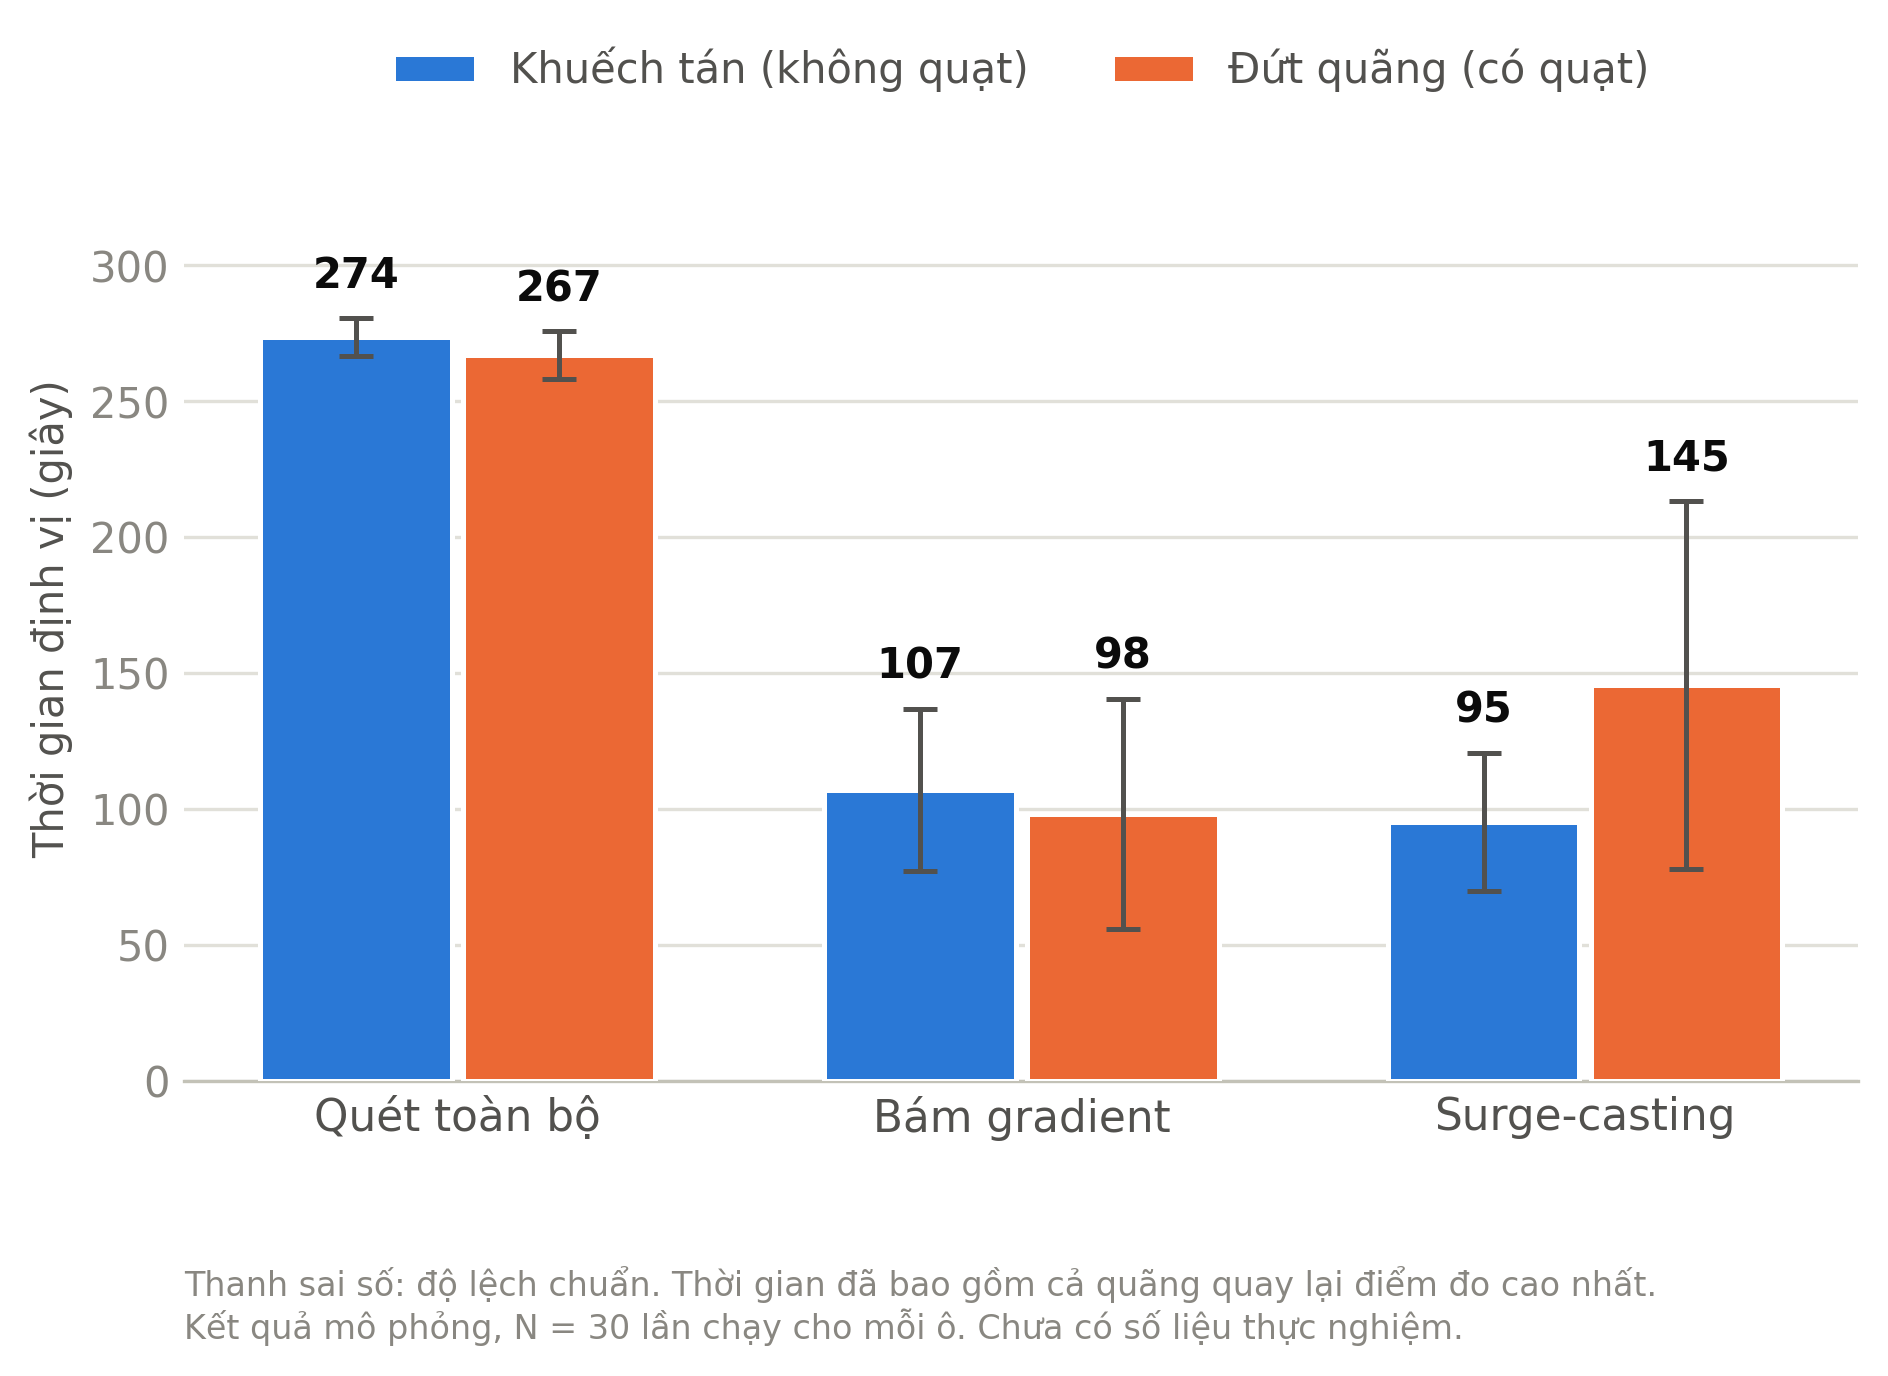
\includegraphics[width=0.912\textwidth]{pic/kq2_thoigian.png}
  \caption{Thời gian định vị trung bình của ba thuật toán trong hai môi trường. Thời gian đã bao gồm cả quãng quay lại điểm đo cao nhất.}
\end{figure}
Hình 6.2 so sánh thời gian định vị. Quét toàn bộ mất khoảng \textbf{270 giây} trong cả hai môi trường, gần như không phụ thuộc môi trường --- đúng như bản chất của nó: thời gian tỉ lệ với số ô phải quét chứ không phụ thuộc vào vị trí nguồn hay cấu trúc dòng khí. Độ lệch chuẩn rất nhỏ (7--9 giây) xác nhận điều này.

Hai thuật toán còn lại nhanh hơn đáng kể. Trong môi trường đứt quãng, surge-casting mất \textbf{145,5 giây}, tức khoảng \textbf{55 \%} thời gian của quét toàn bộ, trong khi đạt tỉ lệ thành công tương đương về mặt thống kê. Trong môi trường khuếch tán, bám gradient mất \textbf{106,8 giây}, tức khoảng \textbf{39 \%} thời gian của quét toàn bộ, cũng với tỉ lệ thành công tương đương về mặt thống kê. Đây chính là giá trị thực tế của hai thuật toán có suy luận: \textbf{cùng độ tin cậy, một nửa tới hai phần năm thời gian}.

\begin{ghichu}
\textbf{Một cảnh báo quan trọng khi đọc bảng:} không được đọc riêng cột thời gian. Bám gradient có thời gian \textbf{ngắn nhất} trong môi trường đứt quãng (98,0 giây), nhưng đó \textbf{không phải ưu điểm} --- nó ngắn vì thuật toán \textbf{kết luận sai sớm}. Một thuật toán dừng nhanh ở nhầm chỗ không phải là một thuật toán nhanh. Vì vậy cột thời gian và cột tỉ lệ thành công phải luôn được đọc cùng nhau.
\end{ghichu}
Cột quãng đường trong Bảng 6.1 củng cố nhận xét trên: bám gradient trong môi trường đứt quãng chỉ đi 4,43 m rồi dừng, trong khi surge-casting đi 9,16 m --- gấp đôi. Surge-casting đi nhiều hơn vì nó \textbf{kiên trì hơn}: mỗi lần mất tín hiệu, nó quét ngang để bắt lại thay vì kết luận vội.


\subsection{Phân bố sai số định vị}
\begin{figure}[!htbp]
  \centering
  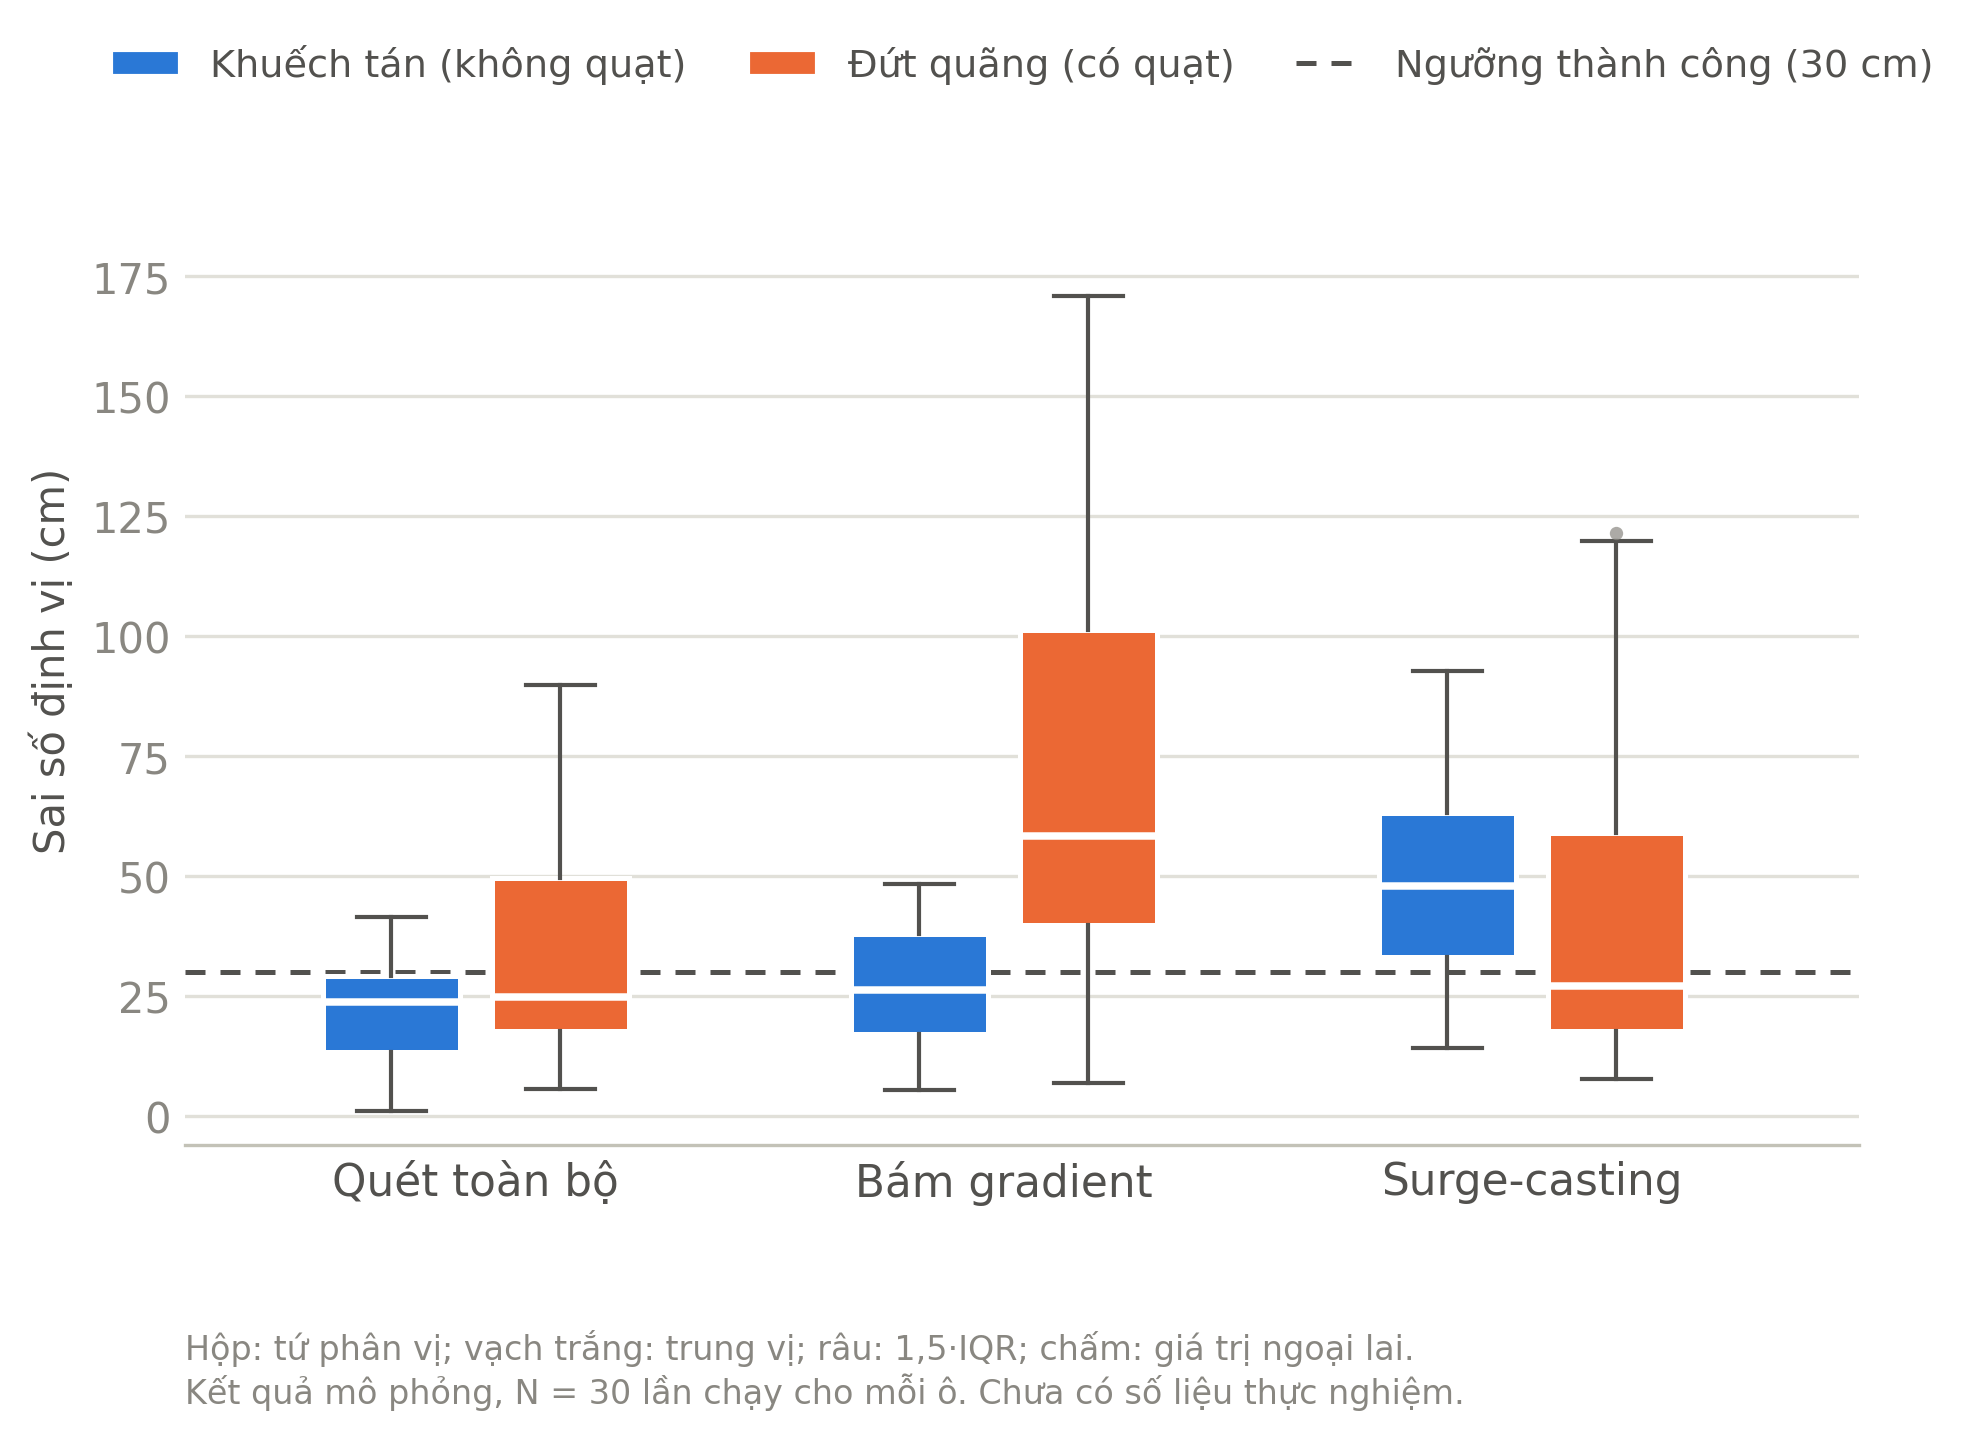
\includegraphics[width=0.912\textwidth]{pic/kq3_saiso.png}
  \caption{Phân bố sai số định vị. Đường đứt nét là ngưỡng thành công 30 cm.}
\end{figure}
Hình 6.3 bổ sung một thông tin mà tỉ lệ thành công không thể hiện được: \textbf{hình dạng của phân bố sai số}, tức là khi thất bại thì thất bại nặng đến mức nào.

Trong môi trường khuếch tán, cả quét toàn bộ và bám gradient có phân bố \textbf{hẹp và nằm gần ngưỡng}: trung vị lần lượt khoảng 23 cm và 26 cm, râu trên không vượt quá 50 cm. Nghĩa là ngay cả khi trượt, chúng cũng trượt không xa.

Trong môi trường đứt quãng, bám gradient có phân bố \textbf{rộng nhất trong toàn bộ thí nghiệm}: trung vị khoảng 59 cm, tứ phân vị trên tới hơn 100 cm và giá trị lớn nhất vượt 170 cm --- tức là gần bằng kích thước cả sân. Đây là dấu hiệu điển hình của một thuật toán bị dẫn đi sai hướng chứ không phải chỉ dừng hơi sớm: nó không lang thang gần nguồn rồi kết luận lệch, nó đi hẳn về một góc khác của sân.

Surge-casting trong môi trường đứt quãng có trung vị khoảng 27 cm, \textbf{nằm ngay dưới ngưỡng thành công}, với hộp tứ phân vị trải từ khoảng 19 tới 59 cm. Phân bố này cho thấy surge-casting thường tới rất gần nguồn, và phần lớn các lần trượt là trượt sát ngưỡng chứ không phải trượt hoàn toàn.


\subsection{Quỹ đạo minh hoạ}
\begin{figure}[!htbp]
  \centering
  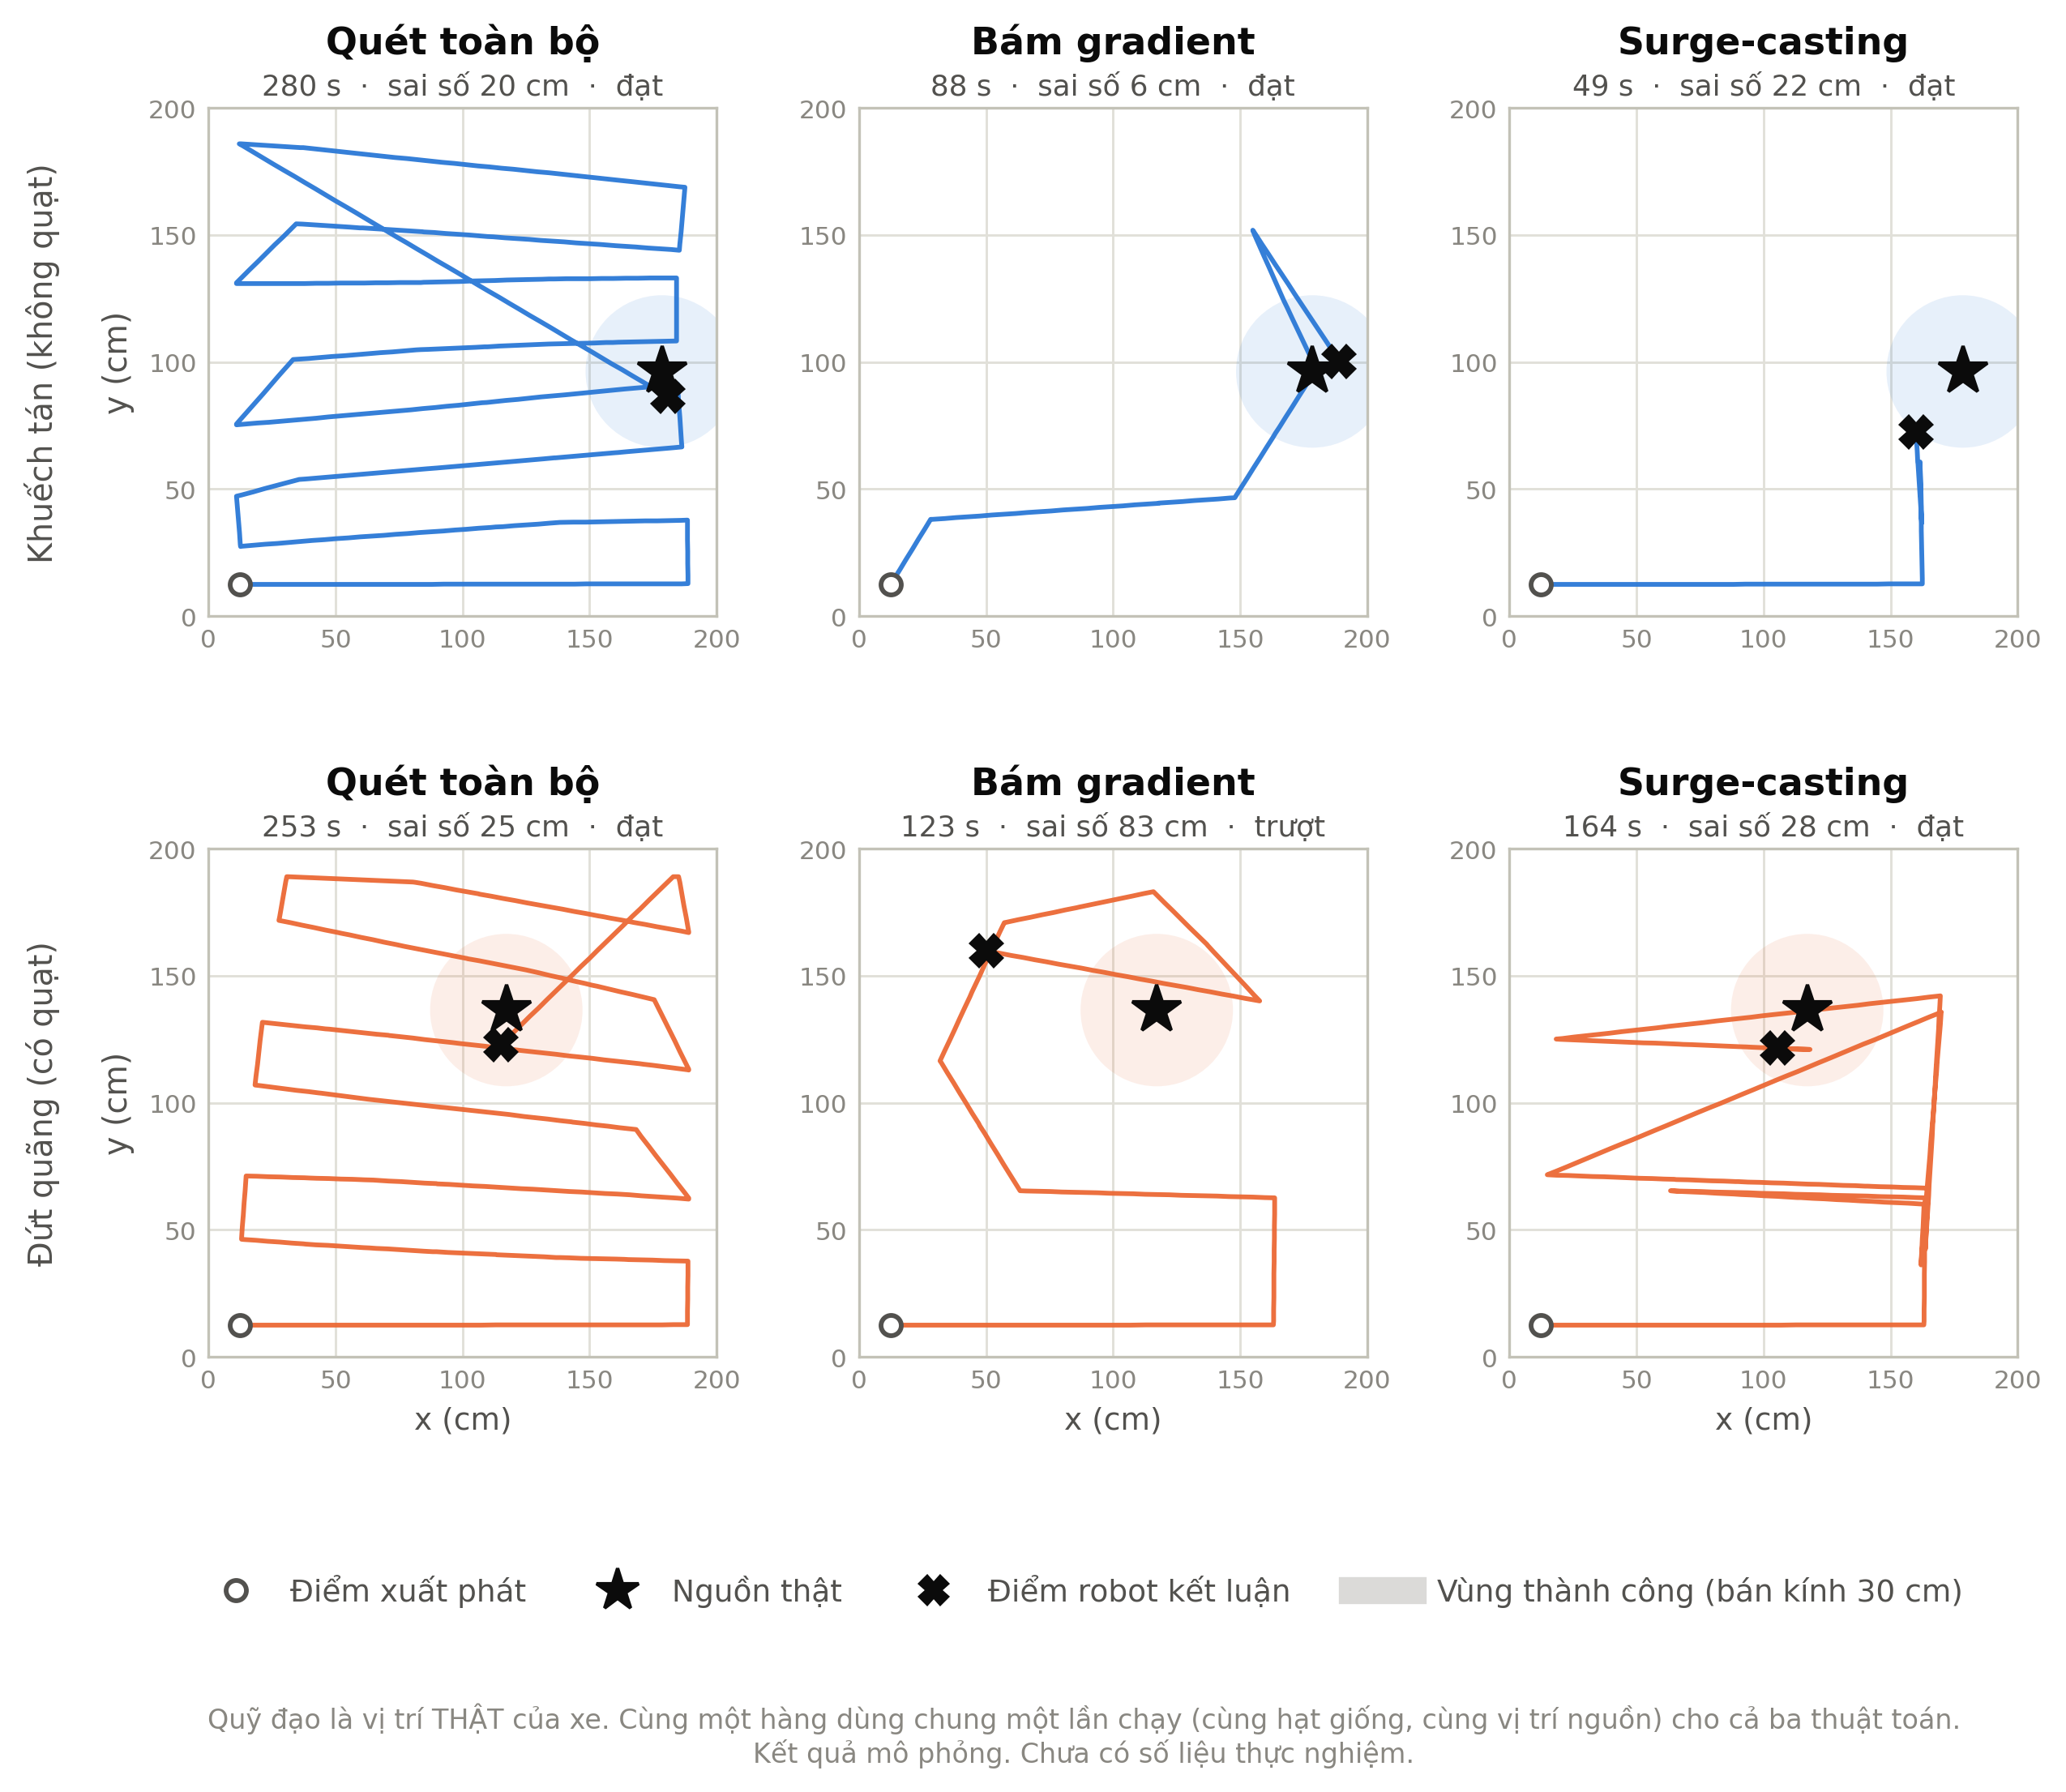
\includegraphics[width=0.941\textwidth]{pic/kq4_quydao.png}
  \caption{Quỹ đạo thật của xe trong hai lần chạy tiêu biểu. Hàng trên: môi trường khuếch tán. Hàng dưới: môi trường đứt quãng. Trong mỗi hàng, cả ba thuật toán gặp cùng một vị trí nguồn.}
\end{figure}
Hình 6.4 minh hoạ trực quan các nhận xét trên.

Ở \textbf{hàng trên (khuếch tán)}, quét toàn bộ đi hết lưới theo đường rắn bò rồi kết luận sau 280 giây với sai số 20 cm. Bám gradient bắt được tín hiệu, đi thẳng gần như trực tiếp tới nguồn và kết luận sau 88 giây với sai số chỉ 6 cm --- đúng hành vi mà H1 dự đoán. Surge-casting cũng kết luận thành công nhưng theo một cách khác hẳn: nó đi thẳng theo hướng gió khai báo cứng, và việc nó tới gần nguồn ở lần chạy này phần nào là do may mắn về hình học.

Ở \textbf{hàng dưới (đứt quãng)}, sự khác biệt rõ hơn nhiều. Quét toàn bộ vẫn quét hết lưới và kết luận đúng. Bám gradient bị các cụm khí rời rạc dẫn lệch hẳn sang trái, kết thúc ở một điểm cách nguồn 83 cm --- một thất bại rõ ràng, đúng như mô tả ở mục 6.4. Surge-casting cho thấy chữ ký hành vi đặc trưng của nó: các đoạn quét ngang biên độ tăng dần đan xen với các đoạn tiến thẳng ngược gió, cuối cùng kết luận cách nguồn 28 cm sau 164 giây.

Một chi tiết đáng chú ý trong quỹ đạo của quét toàn bộ: các hàng quét \textbf{không hoàn toàn song song với trục ngang} mà hơi nghiêng. Đó là biểu hiện trực quan của sai số dead reckoning --- robot tin rằng mình đang đi thẳng theo trục, nhưng vị trí thật lệch dần. Trên toàn bộ 180 lần chạy, độ lệch trung bình giữa vị trí thật và vị trí robot tin là \textbf{7,2 cm}, tương đương khoảng \textbf{0,93 \% quãng đường đã đi}.


\subsection{Kiểm định thống kê}
Với N = 30 cho mỗi ô, các so sánh về tỉ lệ thành công được kiểm định bằng \textbf{kiểm định chính xác Fisher}, còn các so sánh về thời gian được kiểm định bằng \textbf{kiểm định Mann--Whitney U} (không giả định phân phối chuẩn, phù hợp với dữ liệu thời gian lệch phải).

\begin{table}[!htbp]
  \centering
  \caption{Kết quả kiểm định thống kê}
  \small
  \renewcommand{\arraystretch}{1.25}
  \begin{tabular}{>{\raggedright\arraybackslash}p{0.4155\textwidth}>{\raggedright\arraybackslash}p{0.2710\textwidth}>{\raggedright\arraybackslash}p{0.2168\textwidth}}
    \toprule
    \textbf{So sánh} & \textbf{Số liệu} & \textbf{Giá trị \textit{p}} \\
    \midrule
    \textbf{Tỉ lệ thành công --- kiểm định Fisher} &  &  \\
    Bám gradient vs surge-casting, môi trường đứt quãng & 5/30 vs 17/30 & 0,0028 \\
    Bám gradient vs surge-casting, môi trường khuếch tán & 20/30 vs 5/30 & 0,0002 \\
    Quét toàn bộ vs surge-casting, môi trường đứt quãng & 19/30 vs 17/30 & 0,79 \\
    Quét toàn bộ vs bám gradient, môi trường khuếch tán & 23/30 vs 20/30 & 0,57 \\
    \textbf{Ảnh hưởng của môi trường lên từng thuật toán} &  &  \\
    Quét toàn bộ: khuếch tán vs đứt quãng & 23/30 vs 19/30 & 0,40 \\
    Bám gradient: khuếch tán vs đứt quãng & 20/30 vs 5/30 & 0,0002 \\
    Surge-casting: khuếch tán vs đứt quãng & 5/30 vs 17/30 & 0,0028 \\
    \textbf{Thời gian --- kiểm định Mann--Whitney U} &  &  \\
    Surge-casting vs quét toàn bộ, đứt quãng & 138 s vs 266 s (trung vị) & 2,4 $\times$ 10$^{-9}$ \\
    Bám gradient vs quét toàn bộ, khuếch tán & 102 s vs 276 s (trung vị) & 3,0 $\times$ 10$^{-11}$ \\
    \bottomrule
  \end{tabular}
\end{table}
Nhóm ba dòng ở giữa Bảng 6.2 là phần quan trọng nhất và có thể đọc như một khối duy nhất: \textbf{môi trường không ảnh hưởng đáng kể tới quét toàn bộ (\textit{p} = 0,40), nhưng ảnh hưởng rất mạnh và theo hai chiều ngược nhau tới hai thuật toán còn lại (\textit{p} = 0,0002 và \textit{p} = 0,0028).} Đó chính là định nghĩa thống kê của ``không có thuật toán nào thắng ở mọi điều kiện''.

Hai dòng cuối cho thấy lợi thế về thời gian của hai thuật toán có suy luận là \textbf{rất lớn và rất chắc chắn} --- các giá trị \textit{p} nhỏ hơn 10$^{-8}$.

Hai dòng ở giữa phần đầu bảng cũng đáng chú ý theo nghĩa ngược lại: chênh lệch giữa quét toàn bộ và thuật toán ``đúng chỗ'' trong từng môi trường \textbf{không có ý nghĩa thống kê} (\textit{p} = 0,79 và \textit{p} = 0,57). Nghĩa là trong đúng môi trường của mình, hai thuật toán có suy luận đạt độ tin cậy \textbf{ngang với} phương pháp quét vét cạn, nhưng chỉ tốn một phần nhỏ thời gian.


\subsection{Đối chiếu với ba giả thuyết}
\begin{table}[!htbp]
  \centering
  \caption{Đối chiếu kết quả với ba giả thuyết đặt ra ở mục 1.5}
  \small
  \renewcommand{\arraystretch}{1.25}
  \begin{tabular}{>{\raggedright\arraybackslash}p{0.1084\textwidth}>{\raggedright\arraybackslash}p{0.3432\textwidth}>{\raggedright\arraybackslash}p{0.4516\textwidth}}
    \toprule
    \textbf{Giả thuyết} & \textbf{Phát biểu} & \textbf{Kết luận} \\
    \midrule
    H1 & Trong môi trường khuếch tán, bám gradient là thuật toán nhanh nhất & \textbf{Được ủng hộ.} Bám gradient đạt 67 \% thành công trong 106,8 s, so với 17 \% của surge-casting (\textit{p} = 0,0002) và 77 \% của quét toàn bộ trong 273,6 s. Chênh lệch với quét toàn bộ không có ý nghĩa thống kê (\textit{p} = 0,57) nhưng thời gian chỉ bằng 39 \% \\
    H2 & Trong môi trường đứt quãng, surge-casting là thuật toán hiệu quả nhất & \textbf{Được ủng hộ.} Surge-casting đạt 57 \% so với 17 \% của bám gradient (\textit{p} = 0,0028), và ngang với quét toàn bộ về tỉ lệ thành công (\textit{p} = 0,79) trong 55 \% thời gian \\
    H3 & Quét toàn bộ luôn thành công nhưng chậm nhất & \textbf{Chỉ đúng một nửa.} Phần ``chậm nhất'' được xác nhận rõ ràng. Phần ``luôn thành công'' \textbf{bị bác bỏ}: tỉ lệ thực tế là 77 \% và 63 \% \\
    \bottomrule
  \end{tabular}
\end{table}
Bảng 6.3 đối chiếu từng giả thuyết với số liệu thu được. Phần bị bác bỏ của H3 xứng đáng được phân tích, vì nó là kết quả bất ngờ nhất của đề tài.

Sai lầm nằm ở chỗ nhóm đã ngầm đồng nhất \textbf{``phủ kín không gian''} với \textbf{``định vị đúng''}. Quét toàn bộ bảo đảm điều thứ nhất: nó đi qua mọi ô, nên không thể bỏ sót vùng nào. Nhưng kết luận cuối cùng của nó không phải là ``ô nào chứa nguồn'' mà là \textbf{``ô nào đọc được giá trị cao nhất''} --- và hai điều đó không đồng nhất, vì hai lý do đã được phân tích ở Chương 2.

Thứ nhất, \textbf{độ trễ của cảm biến}: giá trị đo tại một ô còn mang dư âm của ô vừa đi qua, nên đỉnh đo được bị dịch đi theo chiều chuyển động. Thứ hai, \textbf{dao động rối của trường nồng độ}: trong môi trường đứt quãng, một ô ở xa nguồn có thể tình cờ hứng trọn một cụm khí đậm và đọc được giá trị cao hơn ô nằm ngay cạnh nguồn tại thời điểm ô đó được đo. Đây chính xác là hiện tượng mà Murlis và cộng sự mô tả ở trang 517 [1] --- phân bố nồng độ đỉnh tại các vị trí khác nhau chồng lấn lên nhau.

Bằng chứng số ủng hộ giải thích này nằm ngay trong dữ liệu: sai số của quét toàn bộ tăng từ 22,7 $\pm$ 10,0 cm (khuếch tán) lên 34,2 $\pm$ 23,3 cm (đứt quãng) --- \textbf{độ lệch chuẩn tăng hơn gấp đôi} trong khi thuật toán không hề thay đổi hành vi. Toàn bộ phần tăng đó đến từ môi trường, không đến từ thuật toán.

\begin{ghichu}
Đây là một bài học phương pháp mà nhóm cho là đáng ghi lại: \textbf{một phép quét vét cạn chỉ vét cạn được không gian tìm kiếm, chứ không vét cạn được sai số của phép đo.} Muốn quét toàn bộ đạt gần 100 \%, cần đo mỗi ô nhiều lần rồi lấy trung bình --- nghĩa là phải trả thêm thời gian, chính là tài nguyên mà nó vốn đã tốn nhiều nhất.
\end{ghichu}

\subsection{Quy tắc chọn thuật toán}
\begin{figure}[!htbp]
  \centering
  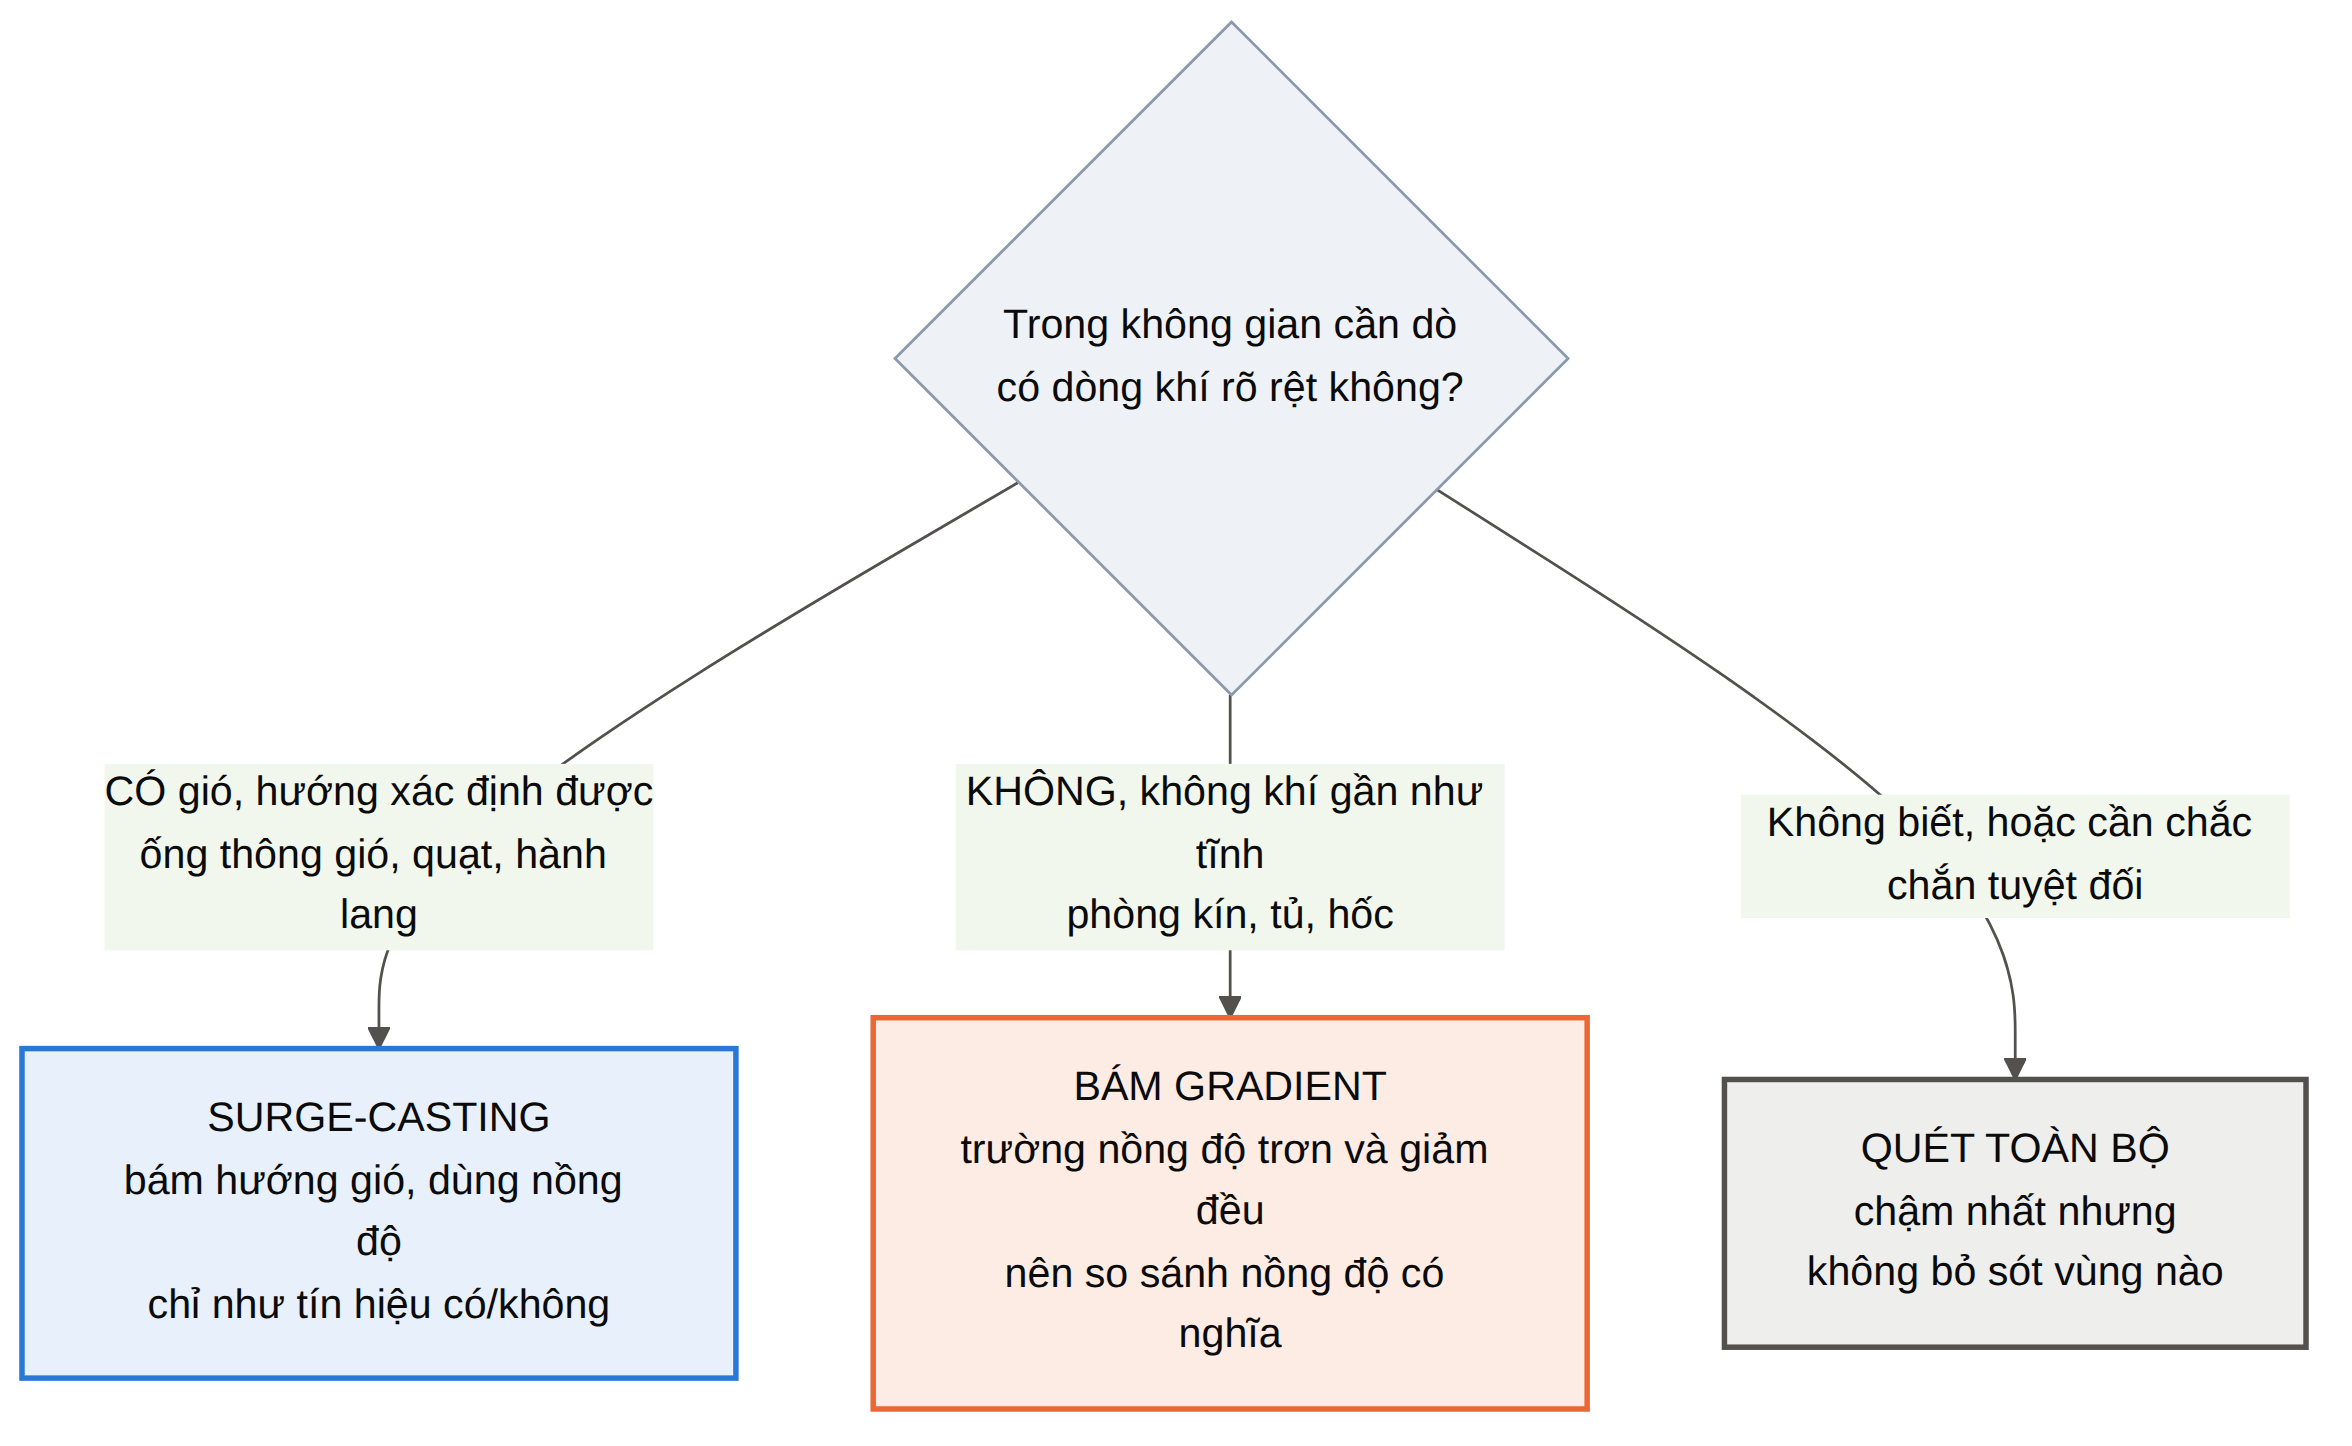
\includegraphics[width=0.941\textwidth]{pic/9_chon_thuat_toan.png}
  \caption{Quy tắc chọn thuật toán theo điều kiện dòng khí.}
\end{figure}
Kết luận có ích của đề tài \textbf{không phải} ``surge-casting là thuật toán tốt nhất'', mà là một quy tắc lựa chọn, tóm tắt ở Hình 6.5:

\begin{itemize}[leftmargin=1.4em,itemsep=0.15em,topsep=0.3em]
  \item \textbf{Nếu môi trường gần như không có gió} và trường nồng độ trơn: dùng \textbf{bám gradient}. Nó nhanh nhất và đạt độ tin cậy ngang phương pháp vét cạn.
  \item \textbf{Nếu môi trường có gió với hướng xác định được}: dùng \textbf{surge-casting}. Bám gradient sẽ thất bại ở đây, còn quét toàn bộ tốn gần gấp đôi thời gian để đạt cùng độ tin cậy.
  \item \textbf{Nếu không biết gì về điều kiện dòng khí}, hoặc nếu độ tin cậy quan trọng hơn thời gian: dùng \textbf{quét toàn bộ}. Nó là thuật toán duy nhất có hiệu năng \textbf{không phụ thuộc môi trường} (\textit{p} = 0,40), tức là thuật toán duy nhất dự đoán được trước.
\end{itemize}
Nhận xét cuối cùng dẫn tới một hệ quả thực tiễn: một hệ thống hoàn chỉnh nên \textbf{đo hướng gió trước, rồi mới chọn thuật toán} --- chứ không nên cố tìm một thuật toán vạn năng. Đây cũng là lý do vì sao việc gắn cảm biến hướng gió được xếp vào nhóm ưu tiên cao trong hướng phát triển.


\subsection{Bàn luận về tính hợp lệ của kết quả}
Nhóm nêu thẳng bốn mối đe doạ tới tính hợp lệ của kết quả trên và cách đã xử lý từng mối.

\textbf{Một --- kết quả có thể phụ thuộc vào bộ tham số mô phỏng.} Đây là mối đe doạ nghiêm trọng nhất và \textbf{chưa được xử lý đầy đủ}. Biện pháp đúng là phân tích độ nhạy như mô tả ở mục 5.5. Nhóm ghi nhận đây là việc chưa hoàn thành. Điều nhóm có thể nói chắc là kết luận được trình bày dưới dạng \textbf{thứ hạng} chứ không phải con số tuyệt đối, và thứ hạng là loại kết luận ít nhạy với tham số nhất.

\textbf{Hai --- mô hình mô phỏng do chính nhóm viết.} Đúng, và vì vậy nó \textbf{không thể được dùng làm bằng chứng thực nghiệm} cho ba giả thuyết. Điều nó chứng minh được đã được phát biểu chính xác ở mục 5.5: với mọi yếu tố ngoài thuật toán được giữ giống hệt nhau, chênh lệch quan sát được chỉ có thể quy cho thuật toán. Điều làm cho kết luận này có giá trị vượt ra ngoài phạm vi mô phỏng là \textbf{cơ chế vật lý dẫn tới nó đã được công bố độc lập trong tài liệu} ([1] cho cấu trúc đứt quãng, [3] cho độ trễ cảm biến): mô phỏng cho thấy hệ quả đúng như cơ chế đã biết dự đoán, chứ không phát hiện ra một hiện tượng mới không có cơ sở.

\textbf{Ba --- hai thuật toán dùng chung giai đoạn dò tìm ban đầu.} Đây là một lựa chọn có chủ ý được nêu ở mục 4.6. Nó làm cho so sánh \textbf{công bằng hơn} ở phần mà H1 và H2 nói tới (hành vi sau khi bắt được luồng khí), nhưng đồng thời cũng có nghĩa là bảng kết quả \textbf{không} đánh giá khả năng dò mù của hai thuật toán. Đó là một giới hạn về phạm vi kết luận, cần được nêu khi trích dẫn kết quả.

\textbf{Bốn --- chưa có số liệu thực nghiệm.} Đây là hạn chế lớn nhất của báo cáo và được nêu lại đầy đủ ở mục 7.2.
